\begin{frame}[plain]
  \begin{center}
    \vspace{2em}
    {\LARGE\textbf{Vision-Language Models}}
  \end{center}
\end{frame}

\begin{frame}{CLIP: Contrastive Language-Image Pretraining}
  \begin{itemize}
    \item[] \textbf{Developed by OpenAI (Radford et al., 2021)}
    \vspace{0.6em}
    \item Trained on 400M (image, text) pairs
    \item Learns a joint embedding space using contrastive loss
    \item Image and text encoders are trained to match correct pairs
  \end{itemize}
  
  \vspace{0.7em}
  \textbf{Use cases:}
  \begin{itemize}
    \item Zero-shot classification
    \item Semantic similarity
    \item Prompt-based image querying
  \end{itemize}
\end{frame}

\begin{frame}{CLIP: Contrastive Language-Image Pretraining \hfill \includegraphics[height=1em]{assets/KAUST_logo.png}}
  \textbf{Architecture:}
  \begin{itemize}
    \item[{\color{red}\textbullet}] ResNet / ViT for images
    \item[{\color{red}\textbullet}] Transformer for text
    \item[{\color{red}\textbullet}] Cosine similarity loss
  \end{itemize}

  \vspace{1em}
  \textbf{Paper:}
  \href{https://arxiv.org/abs/2103.00020}{\colorbox{yellow!20}{CLIP: Learning Transferable Visual Models From Natural Language Supervision}}
  \hspace{0.5em}
  {\scriptsize\ttfamily https://arxiv.org/abs/2103.00020}
\end{frame}

\begin{frame}{CLIP (Radford et al. 2021)}
  \begin{itemize}
    \item \textbf{Exact same contrastive loss as earlier, but with Transformers and "web data"!}
  \end{itemize}
  \vspace{1em}
  % Placeholder for architecture diagram
  \begin{center}
    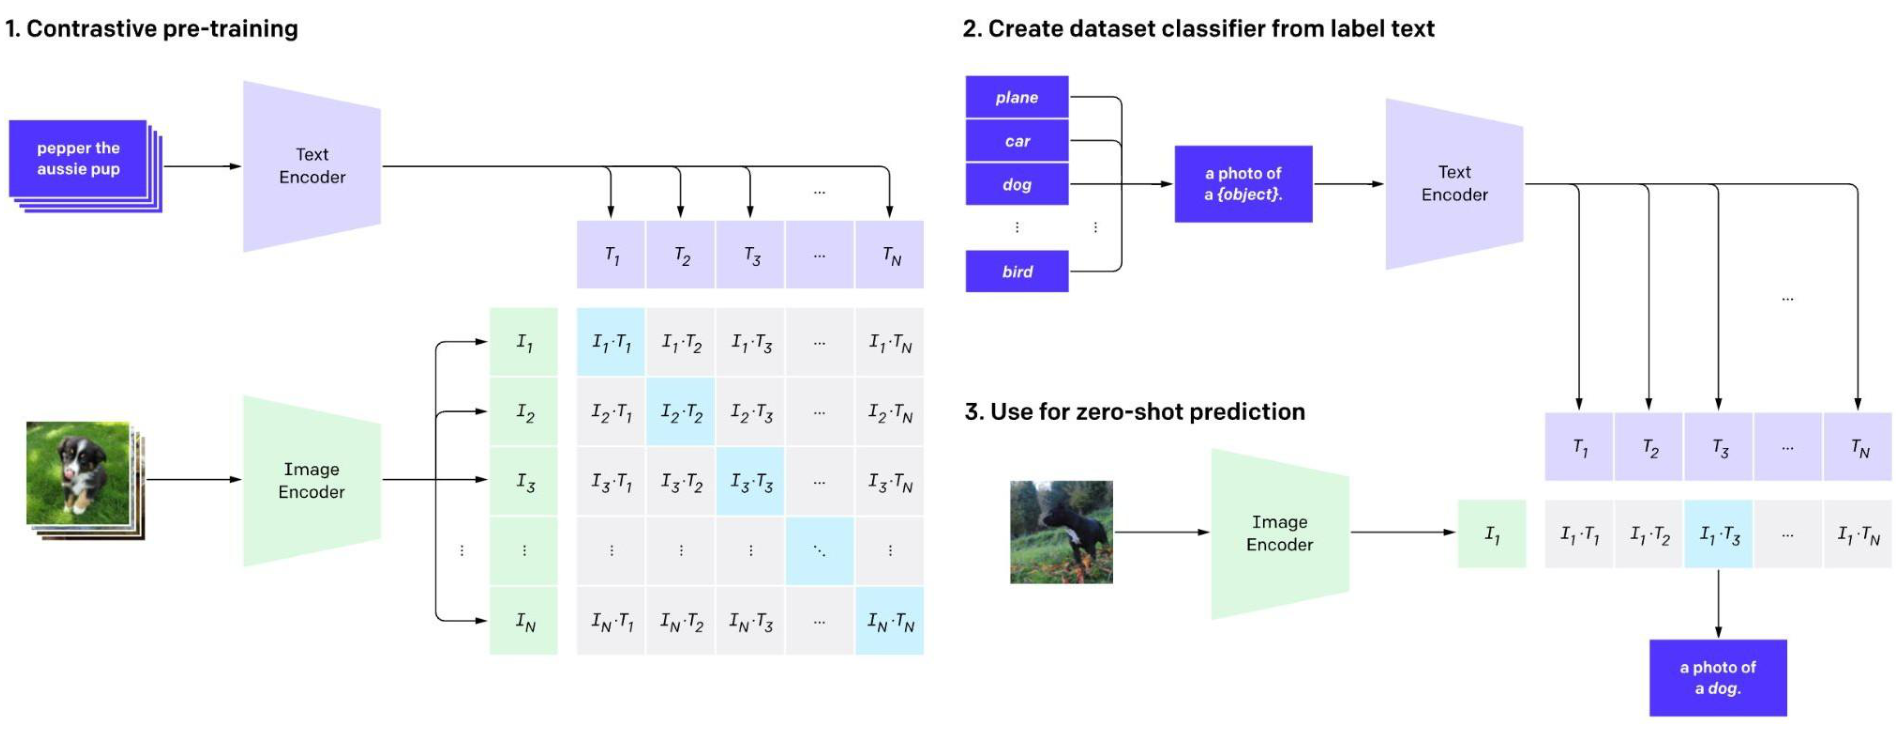
\includegraphics[width=0.9\textwidth, height=0.9\textheight, keepaspectratio]{assets/Lecture-10_Multimodal_NLP_Agentic_AI/slide_012.png}  
  \end{center}
\end{frame}

\begin{frame}{CLIP Robustness}
  \begin{itemize}
    \item \textbf{IMHO one of the best papers ever written in our field: extremely thorough, worth a close read.}
    \vspace{0.7em}
    \item Generalizes \textbf{MUCH} better~$\rightarrow$
  \end{itemize}
  \vspace{1em}
  \begin{center}
    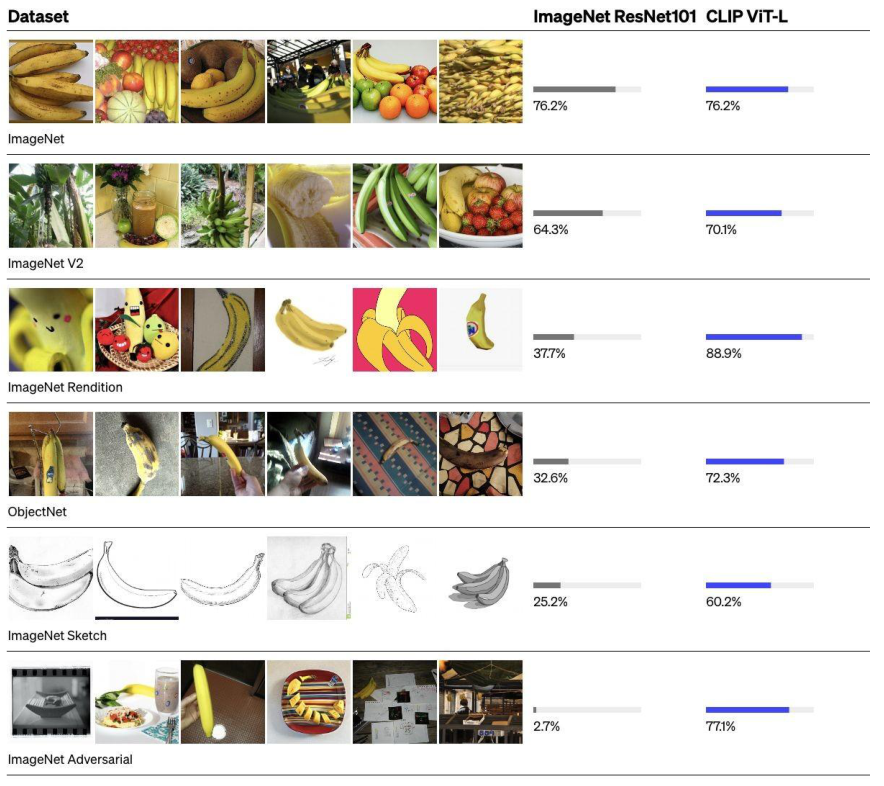
\includegraphics[width=0.65\textwidth, height=0.65\textheight, keepaspectratio]{assets/Lecture-10_Multimodal_NLP_Agentic_AI/slide_013.png}
  \end{center}
  % Replace with higher-res crop of robustness table if possible
\end{frame}

\begin{frame}{VisualBERT: Overview}
  \begin{itemize}
    \item[{\color{red}\textbullet}] \textbf{Joint Transformer-based model:} processes both image regions and text.
    \item[{\color{red}\textbullet}] \textbf{Early fusion:} image embeddings are added as input tokens to the Transformer.
    \item[{\color{red}\textbullet}] \textbf{Pretraining objectives:}
    \begin{itemize}
      \item Masked Language Modeling (MLM)
      \item Next Sentence Prediction (NSP)
      \item Image-Text Alignment
    \end{itemize}
  \end{itemize}
\end{frame}

\begin{frame}{VisualBERT: Applications and Reference}
  \textbf{Applications:}
  \begin{itemize}
    \item Visual Question Answering (VQA)
    \item Image captioning
    \item Visual commonsense reasoning
  \end{itemize}

  \vspace{0.7em}
  \textbf{Paper:}
  \href{https://arxiv.org/abs/1908.03557}{\colorbox{pink!20}{VisualBERT: A Simple and Performant Baseline for Vision and Language}}
  \hspace{0.5em}
  {\scriptsize\ttfamily https://arxiv.org/abs/1908.03557}
\end{frame}

\begin{frame}{VisualBERTs: VisualBERT Architecture}
  \begin{center}
    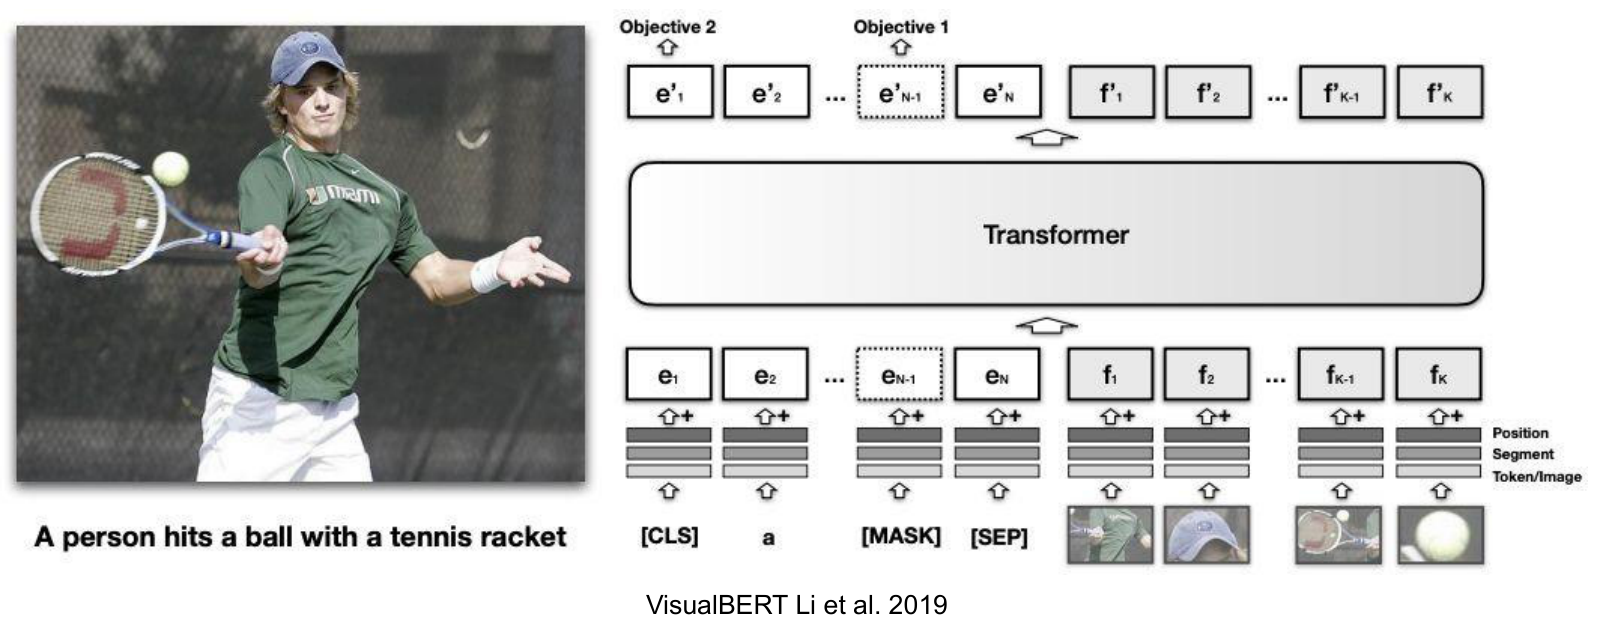
\includegraphics[width=0.98\textwidth, height=0.98\textheight, keepaspectratio]{assets/Lecture-10_Multimodal_NLP_Agentic_AI/slide_015.png}
  \end{center}  
\end{frame}

\begin{frame}{Visual BERTs: ViLBERT}
  \begin{center}
    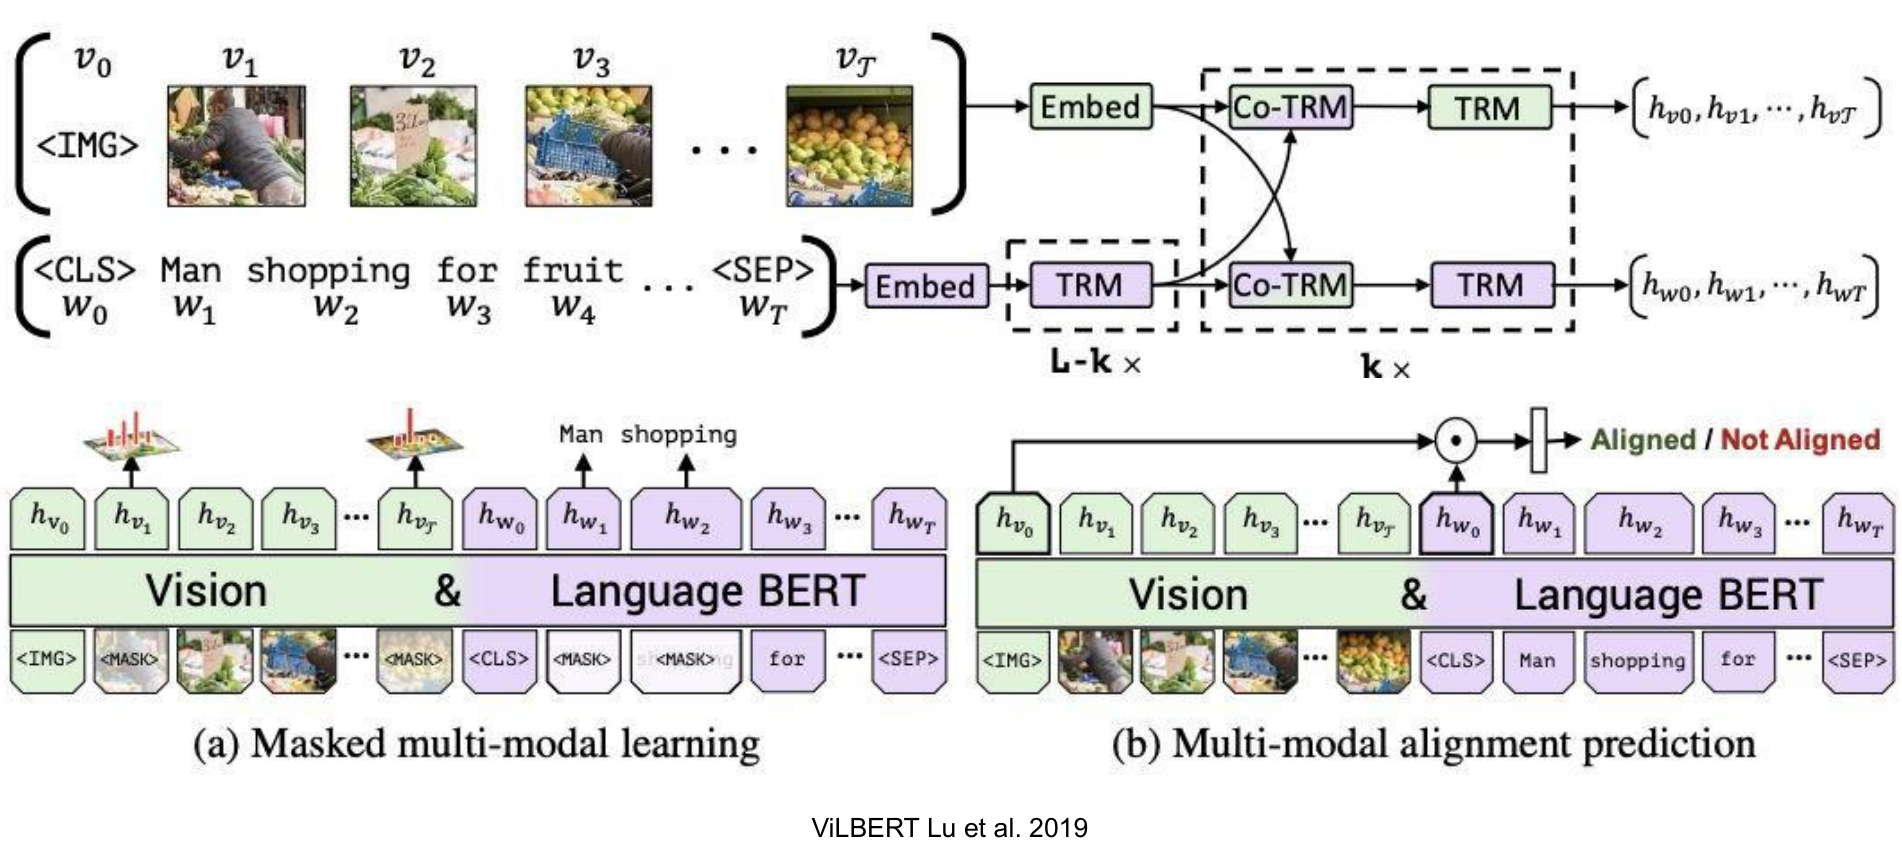
\includegraphics[width=0.98\textwidth, height=0.98\textheight, keepaspectratio]{assets/Lecture-10_Multimodal_NLP_Agentic_AI/slide_016.png}
  \end{center}  
\end{frame}

\begin{frame}{Visual BERTs: LXMERT}
  \textbf{LXMERT: Learning Cross-Modality Encoder Representations from Transformers}
  \begin{center}
    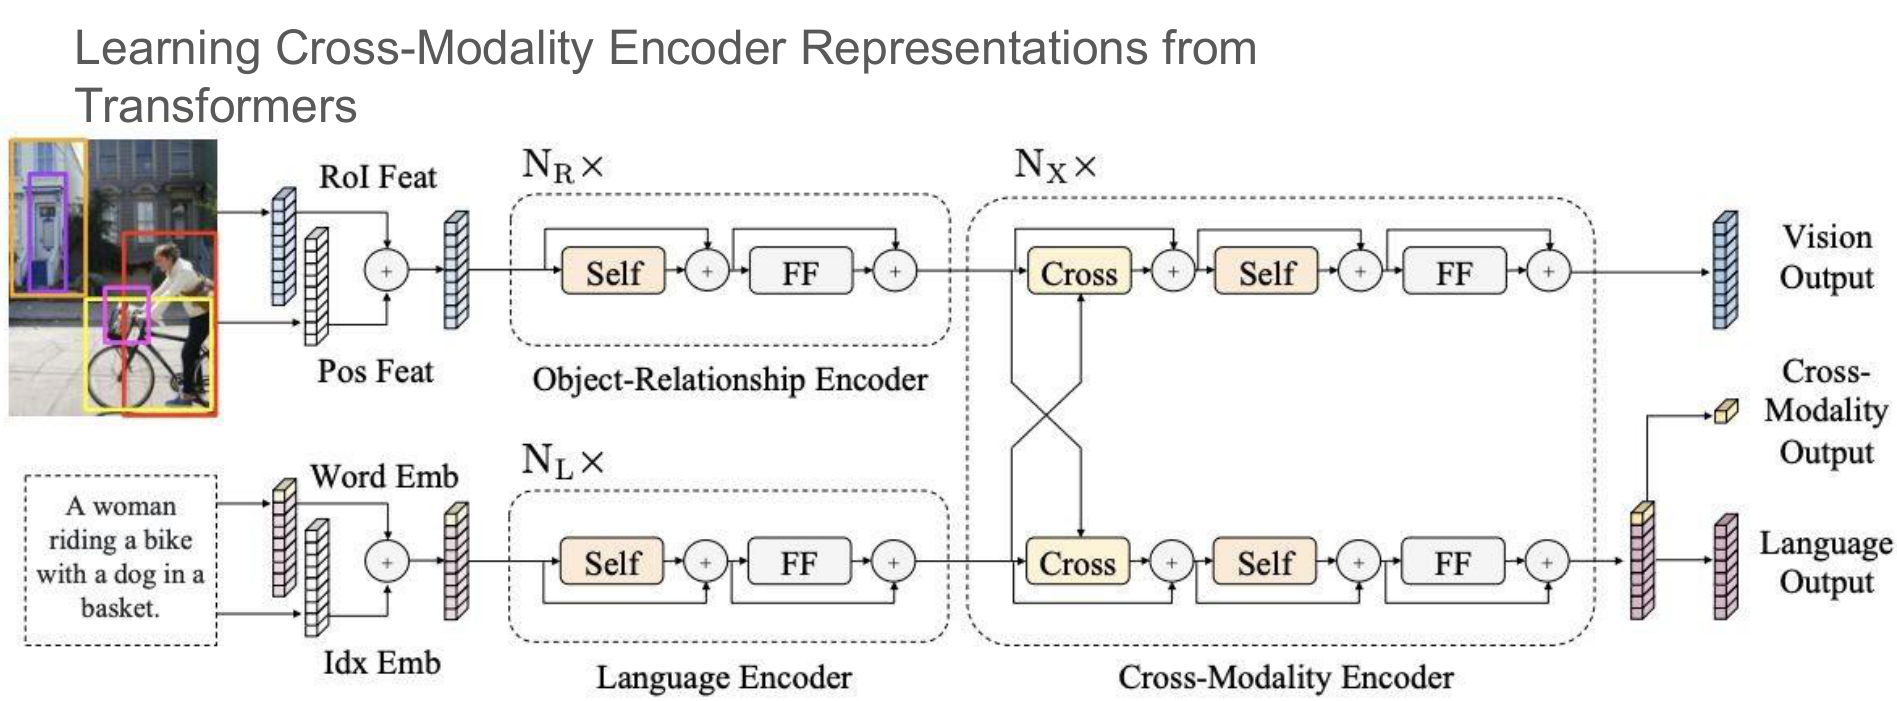
\includegraphics[width=0.92\textwidth, height=0.92\textheight, keepaspectratio]{assets/Lecture-10_Multimodal_NLP_Agentic_AI/slide_017.png}
    \tiny{\hspace{0.5em} LXMERT Tan \& Bansal 2019}
  \end{center}
\end{frame}

\begin{frame}{Visual BERTs: Supervised Multimodal Bitransformers}
  % [Placeholder for image: Illustration of the multimodal bitransformer architecture as in slide_018.png or corresponding asset]
  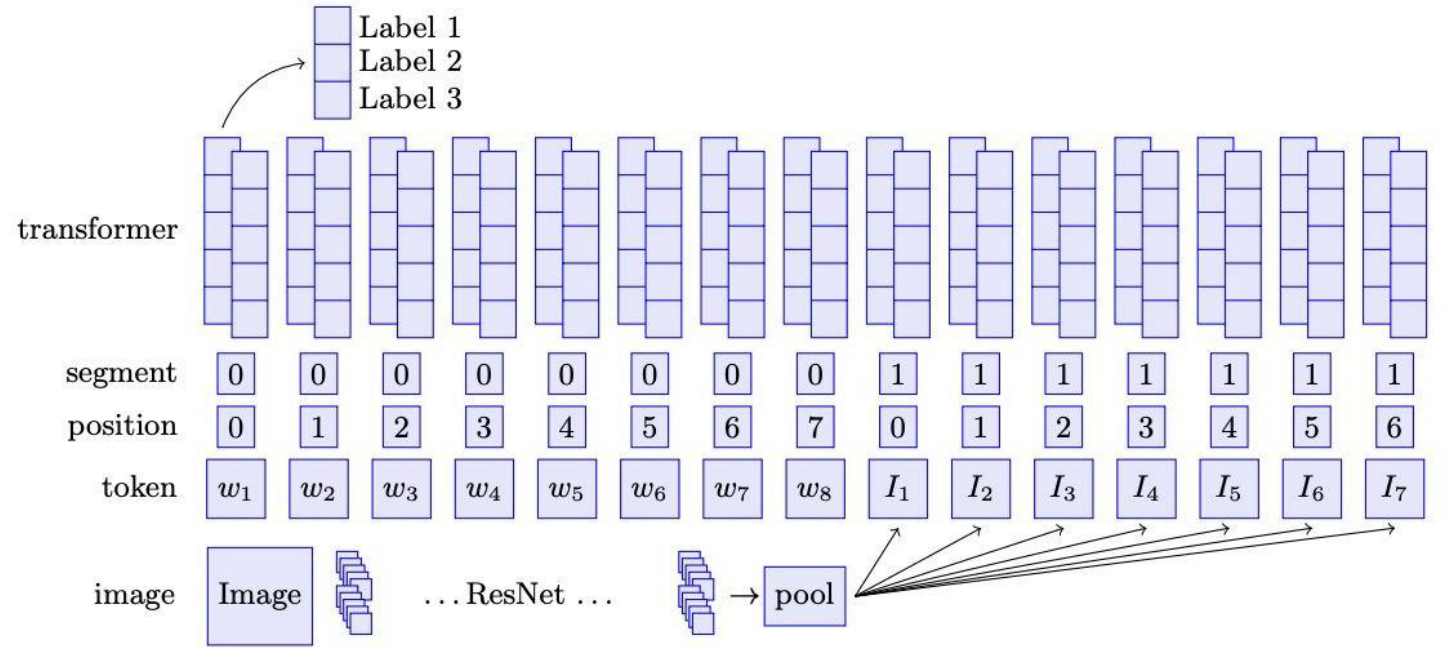
\includegraphics[width=0.98\textwidth, height=0.6\textheight, keepaspectratio]{assets/Lecture-10_Multimodal_NLP_Agentic_AI/slide_018.png}
  
  % \begin{itemize}
  %   \item \textbf{Description:} 
  %     This diagram illustrates the multimodal bitransformer architecture. It shows how input tokens and image features, extracted (e.g., via ResNet and pooling), are fed into a shared transformer, with associated segment, position, and token embeddings, to enable supervised multimodal learning.
  %   \item \textbf{Reference:} 
  %     {\small MMBT (Kiela et al., 2019)}
  % \end{itemize}

  \vspace{1em}
  \centering
  {\scriptsize Figure 1: Illustration of the multimodal bitransformer architecture.\\
  MMBT Kiela et al. 2019}
\end{frame}

\begin{frame}{Visual BERTs: PixelBert}
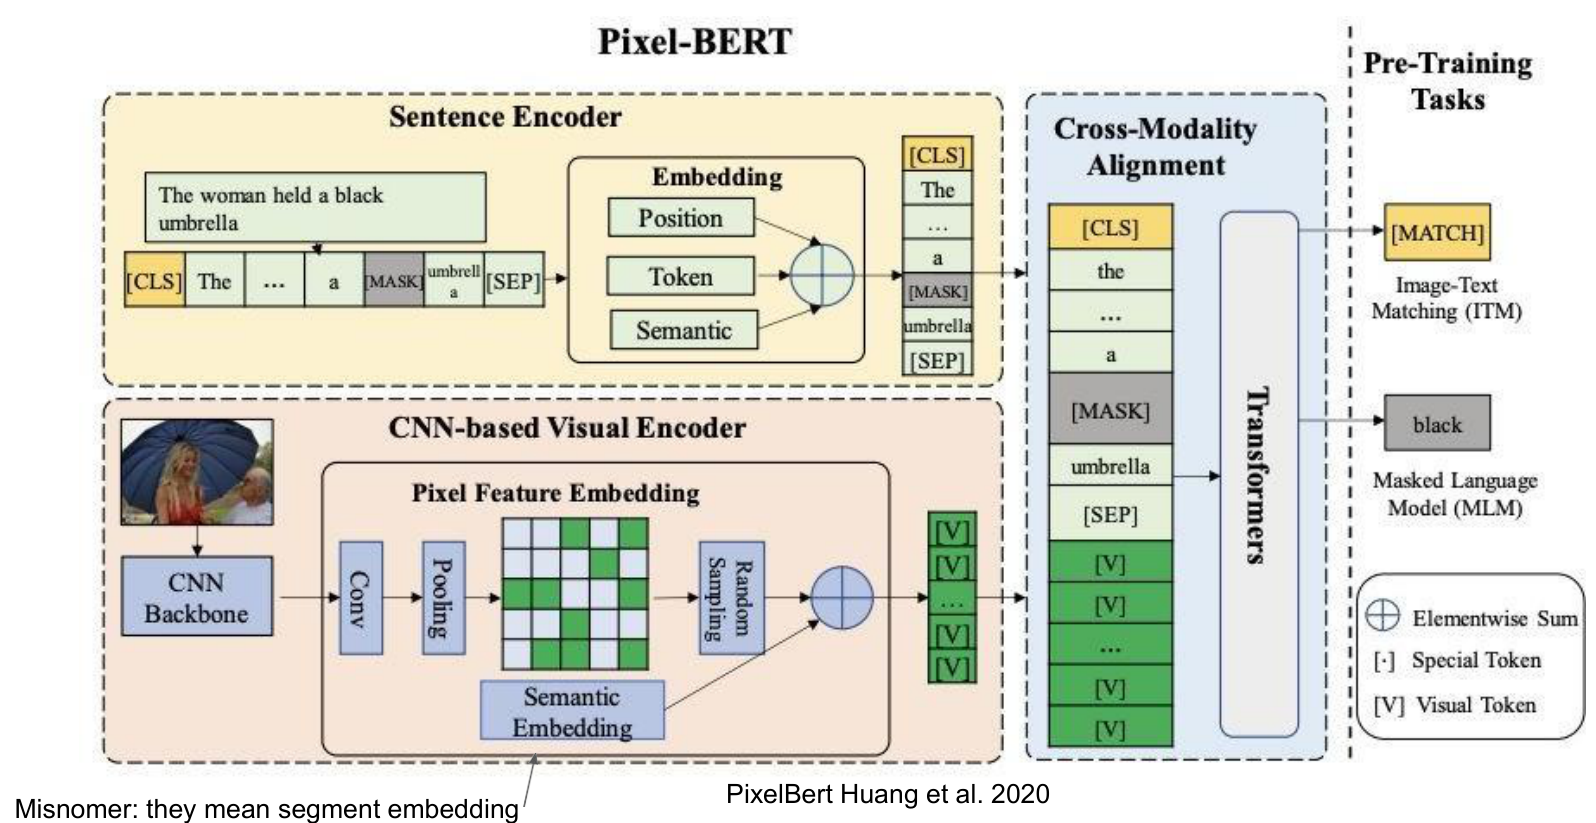
\includegraphics[width=0.98\textwidth, height=0.98\textheight, keepaspectratio]{assets/Lecture-10_Multimodal_NLP_Agentic_AI/slide_019.png}
\end{frame}

\begin{frame}{FLAVA (Facebook AI)}
  \begin{itemize}
    \item \textbf{FLAVA = Fusion of Language And Vision Architecture}
    \item Handles both unimodal and multimodal tasks
    \item \textbf{Three towers:} vision, language, multimodal
    \item Self-supervised objectives: masked modeling, contrastive learning
  \end{itemize}

  \vspace{0.7em}
  \textbf{Capabilities:}
  \begin{itemize}
    \item Text classification
    \item Image classification
    \item Visual Question Answering (VQA)
    \item Image captioning
  \end{itemize}
  
  \vspace{0.7em}
  \textbf{Paper:}
  \href{https://arxiv.org/abs/2112.04482}{\colorbox{pink!20}{FLAVA: A Foundational Language And Vision Alignment Model}}
  \hspace{0.5em}
  {\scriptsize\ttfamily https://arxiv.org/abs/2112.04482}
\end{frame}

\begin{frame}{FLAVA (Singh et al., 2021)}
  \begin{columns}
    \begin{column}{0.58\textwidth}
      Holistic approach to multimodality.\\
      One foundation model spanning V\&L, CV and NLP.\\
      Jointly pre-trained on:
      \begin{itemize}
        \item unimodal text data (CCNews + BookCorpus)
        \item unimodal image data (ImageNet)
        \item public paired image-text data (70M)
      \end{itemize}
      All data/models are publicly released.
    \end{column}
    \begin{column}{0.40\textwidth}
      % Placeholder for image (slide_020.png)
      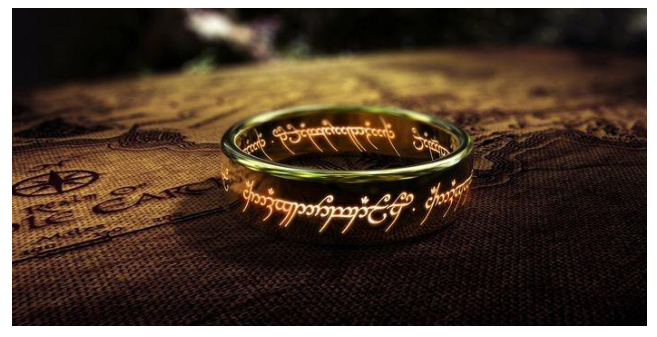
\includegraphics[width=\textwidth]{assets/Lecture-10_Multimodal_NLP_Agentic_AI/slide_021.png}
    \end{column}
  \end{columns}
\end{frame}
